\documentclass[conference]{IEEEtran}
\IEEEoverridecommandlockouts
\IEEEpubid{\makebox[\textwidth]{\textbf{978-1-6654-5122-2/22/\$31.00~\copyright2022 IEEE} \hfill}}

\usepackage{cite}
\usepackage{amsmath,amssymb,amsfonts}
\usepackage{multirow}
\usepackage{multicol}
\usepackage{graphicx}
\usepackage{textcomp}
\usepackage{xcolor}
\usepackage{array}
\usepackage{tabularx}
% \usepackage{float}

% folder gambar
\graphicspath{{./figures/}}

\newcolumntype{M}[1]{>{\centering\arraybackslash}m{#1}}

\renewcommand\IEEEkeywordsname{keywords}

\begin{document}

\title{Effects of Ground Trimming and Feedline Extension in Designing A Microstrip Patch Antenna for RF Applications}

\author{
\IEEEauthorblockN{Muhammad Ogin Hasanuddin\IEEEauthorrefmark{2}, Christian Dinata, Ahmad Izzuddin}
\IEEEauthorblockA{\textit{School of Electrical Engineering and Informatics} \\
\textit{Bandung Institute of Technology}\\
Bandung, Indonesia \\
Corresponding author: \IEEEauthorrefmark{2}moginh@itb.ac.id}
}



\maketitle
\IEEEpubidadjcol

\begin{abstract}
  Radio-frequency energy harvesting (RFEH) has attracted significant interest as one of the methods of enabling a battery-free sustainable wireless IoT system. Rectenna comes in handy in scavenging an amount of energy at a specific range of frequency, radiation-to-ac harvesting. In that sense, however, not a single antenna managed to perform perfectly for various distinct cases and even in its own one considering its limitations and dynamic parameters. This study proposed a microstrip patch antenna that is designed particularly to operate at 915 MHz frequency utilizing the ground trimming and feedline extension technique to cover the changes of the printed one's parameter. The analysis of the 79.1 mm $\times$ 69 mm microstrip patch antenna showed a return loss of -16.664 dB and a VSWR of 1.3437 at a frequency of 915 MHz. The implemented antenna has a wide operating frequency from 742.21 MHz to 1549.2 MHz although it has a higher input impedance of 56.3 ohms. In conclusion, this antenna can work with various RFEH sources at a wider frequency band.
\end{abstract}

\begin{IEEEkeywords}
  rectenna, return loss, VSWR, Wide frequency band, RFEH
\end{IEEEkeywords}

\section{Introduction}
As we know, now we live in the era where radio frequency become vital in the environment around us, such as the use of electronic gate toll, health monitoring, and even in education. In the environment around us, we can "harvest" tiny amounts of dissipating energy from radio frequency signals and use it as available electric energy. This technology is known as energy harvesting. Energy harvesting is a vast and rapidly growing industry. At 2015, energy harvesting system market was estimated worth \$8 billion by 2020 \cite{popresearch}, and today it was estimated worth \$15.01 billion by 2028. No wonder energy harvesting has been implemented at most papers as the alternative of a battery-free sustainable wireless system since it is actually impossible to keep replacing the batteries connected to sensors many times. There are various sources of energy harvesting from the ambient environment which are solar sources \cite{baccouch2016patch}, thermal sources \cite{kishore2018review}, mechanical vibrations \cite{wei2017comprehensive}, and radio frequency. Despite the characteristics of each energy harvesting source, the radio frequency has the lowest power density but it appears to always present throughout the day. This term is often known as Radio Frequency Energy Harvesting (RFEH). 

One of the main technology used in harvesting the energy of radio frequency is antenna. In this context, antenna can be used to collect an amount of energy from the ambient environment which is the radio-frequency signal and forward 100\% of the collected in ideal case in the order of dBm to the feedline that is connected to a rectifier. The challenge that often occurs to antenna designer is how to actually design a particular antenna that works the way it's planned to. Surely there are various types of antennas but one of the most effective types of antennas in radio-frequency energy harvesting is the microstrip patch antenna. 

The rating performance of an antenna is fundamentally based on how it is designed and implemented. Nonetheless, in the real world, antennas hardly performed as what the designers wanted to since it has a dynamic parameter that is not universally union in value for example, the dielectric constant of the material used. Hence, this paper proposed two out of various techniques that are proven to be plausible ways in enhancing the performance of an antenna. The techniques that are going to be implemented in designing a microstrip patch antenna are ground trimming and feedline extension. This microstrip patch antenna is expected to work at 915 MHz frequency for the purpose of the radio-frequency energy harvesting. 

\section{Related Works}
Due to the high demand in RF energy harvesting field, there have been several previous attempts to design an antenna module. Most of the antennas that are used for this purpose are the microstrip patch antenna. However, microstrip patch antenna has a narrow bandwidth and so there have been several techniques implemented in enhancing the antenna.  

Recent study proposed an antenna bandwidth enhancement by adding a U-shape slot on the patch~\cite{surmeli2011u}. The U-slot behaves as a serial capacitor thus the inductive behaviour of probe feed can be compensated and impedance matching can be obtained. It's proven to be able to increase the bandwidth of 30\%. However, due to the various shapes of slots and parameters, this technique is a little bit more complex and suitable only for specific values of substrate permittivity and thickness.

Another attempt involved a modification of a rectangular microstrip patch antenna using truncated corner technique~\cite{armin2020modification}. This technique is done by cutting the edge of the top and bottom of the patch in a calculated degree which in this case is 45 degrees. Thus, the antenna will resonant at two different frequencies because there are two different diagonal lengths. It's proven to be effective to create a circular polarization nonetheless for the bandwidth side, two or more resonant frequencies is different to a wideband frequency. 

Rather than modifying the patch, another study proposed a technique that is called a taper matching feedline~\cite{rabbani2014simple}. Essentially, the feedline of the microstrip patch antenna is needed to be reshaped into a taper shape that forms sort of a triangle. This is a simple approach in enhancing the antenna performance however, it doesn't enhance that much. The study showed that the antenna bandwidth is increased by around 9\% but the return loss is around 35\% better than before the modification.

\section{Design and Implementation}
Essentially, there are two basic steps in creating an antenna which are design and implementation. This study focuses at two main considerations in designing the antenna: Bandwidth and S11 Parameter at 915 MHz. As a matter of fact, there's nothing perfectly created out there in real life, hence, modification techniques are needed. Therefore, this study provided two types of antenna, the original one and the modified one.

\subsection{Antenna Terminology}
The terminology of antenna contains 3 main topics. Those are the material used, expected performance of the antenna, and the calculation formulas. Each of those is described below. 
\begin{itemize}
  \item Substrate: FR-4 (Lossy)
  \item Patch: Copper
  \item Ground plane: Copper
\end{itemize} 

\begin{table}[htbp]
  \begin{center}
  \caption{Antenna Performance Specifications}
  \label{tab:tab1}
  \begin{tabular}{| M{3cm} | M{3cm} |}
    \hline
    \textbf{Parameter} & \textbf{Value} \\
    \hline
    Operating Frequency & 900 - 925 MHz \\
    \hline
    Return Loss & $<$ -10 dB\\ 
    \hline
    VSWR & $<$ -2\\ 
    \hline
    Input Impedance & (50$\pm$ 2) $\Omega$\\
    \hline
  \end{tabular}
  \end{center}
  \end{table}

These formulas are based on the book of Balanis Antenna Theory: Analysis and Design \cite{balanis2015antenna}.

\begin{table}
  \begin{center}
  \caption{Antenna Parameter Formula}
  \label{tab:tab2}
  \begin{tabular}{| M{2cm}| M{5cm} |}
    \hline
    \textbf{Parameter} & \textbf{Formula} \\ 
    \hline
    Patch Length (L) & \[L = \frac{1}{2.f_{r}.\sqrt{\epsilon_{r.eff}}.\sqrt{\mu_{0}.\epsilon_{0}}  }- 2.\Delta L\] \\
    \hline
    Patch Width (W) & \[W = \frac{1}{2.f_{r}.\sqrt{\mu_{0}.\epsilon_{0}}  }.\sqrt{\frac{2}{\epsilon_{r}+1}}\]\\ 
    \hline
    Feedline Total Length ($L_{f}$) & \[L_{f}\approx \frac{L}{2} \]\\
    \hline
    Feedline Total Width ($W_{f}$) & \[W_{f}= \frac{7.48*h}{3.9484} - 1.25-t \]\\ 
    \hline
    Ground Plane Length ($L_{g}$) & \[L_{g} = 6*h+L \]\\ 
    \hline
    Ground Plane Width ($W_{g}$) & \[W_{g} = 6*h+W \]\\ 
    \hline
    Feedline Length (Fi) & $Fi = 10^{-4}.(0.001699*\epsilon_{r}^{7}+0.13761*\epsilon_{r}^{6}-6.17383 * \epsilon_{r}^{5} + 93.187 * \epsilon_{r}^{4}\newline-682.69*\epsilon_{r}^{3} +2561.9*\epsilon_{r}^{2} +\epsilon_{r}+6697)*\frac{L}{2}$ \\ 
    \hline
    Gap Width (Gpf) & \[g = \frac{v_{0}}{\sqrt{2*\epsilon_{eff}}} . \frac{4.65*10^{-12}}{f} \]\\ 
    \hline
  \end{tabular}
  \end{center}
  \end{table}

\subsection{Antenna Version 0}
Antenna version 0 is the first model of antenna that this study proposed which means it has not been modified. The parameter calculations referred to Table~\ref{tab:tab2} and the design result is shown in table~\ref{tab:tab3}. These values were taken objectively based on the simulation in CST Studio.

As what has been shown in Table~\ref{tab:tab3}, the initial values of the antenna parameters unexpectedly resulted a shifted operating frequency range and a bad VSWR ratio value. It happened because the calculations are simplified into a simpler form as what are stated in Balanis Book \cite{balanis2015antenna}. Therefore, in order to optimize the performance of the antenna, we have to tune the antenna using the parameter sweep technique in CST Studio software. Sweeping on the patch length (L) resulted a shifting of the operating frequency. Decreasing the patch length (L) will shift the frequency to the right and vice versa. Sweeping on the patch width (W) will improve the return loss. Decreasing the patch width (W) will lower the return loss which is better and vice versa. To be concise, there are some steps that were done in the sweeps.
\begin{itemize}
  \item Swept the patch length (L) from 76.175 mm to 78.8 mm. Found the optimal result at 76.375 mm.
  \item Swept the patch width (W) from 100.7 mm to 67 mm. Found the optimal result at 69 mm.
  \item Operating frequency shifted a bit because of patch width (W) sweeps, so swept the patch length (L) from 76.375 mm to 77.13 mm. Found the optimal result at 77.13 mm.
\end{itemize} 

\begin{table}
  \begin{center}
  \caption{Antenna Version 0 Initial Specifications}
  \label{tab:tab3}
  \begin{tabular}{| M{2cm}| M{5cm} |}
      \hline
      \textbf{Parameter} & \textbf{Value} \\ 
      \hline
      Patch Length (L) & 78.8 mm \\
      \hline
      Patch Width (W) & 100.7 mm\\ 
      \hline
      Ground Plane Length ($L_{g}$) & 88.4 mm\\ 
      \hline
      Ground Plane Width ($W_{g}$) & 110.25 mm\\ 
      \hline
      Bandwidth & ~13.53 MHz\\ 
      \hline
      Operating Frequency & 880.5 MHz - 894.03 MHz\\ 
      \hline
      Return Loss & -16.162 dB\\ 
      \hline
      VSWR & 7.6764\\ 
      \hline
      Input Impedance & 49.274$\Omega$ \\ 
      \hline
  \end{tabular}
  \end{center}
  \end{table}  

The improved performance of antenna version 0 after all the sweepings which are the return loss, VSWR, and input impedance were obtained and can be seen in CST Studio software. Therefore, final specifications of the optimized antenna version 0 can be seen on Table~\ref{tab:tab4}. As the results, we can see improvements of the operating frequency which has shifted to the higher frequency with the resonant one at 914.95 MHz, VSWR which is now lower than 2, and even a smaller dimension of microstrip patch antenna. 
\begin{table}[htbp]
\begin{center}
\caption{Antenna Version 0 Final Specifications}
\label{tab:tab4}
\begin{tabular}{| M{2cm}| M{5cm} |}
    \hline
    \textbf{Parameter} & \textbf{Value} \\ 
    \hline
    Patch Length (L) & 77.13 mm \\
    \hline
    Patch Width (W) & 69 mm\\ 
    \hline
    Ground Plane Length ($L_{g}$) & 86.73 mm\\ 
    \hline
    Ground Plane Width ($W_{g}$) & 78.6 mm\\
    \hline
    Bandwidth & ~18.29 MHz\\ 
    \hline
    Operating Frequency & 905.9 MHz - 924.19 MHz\\ 
    \hline
    Return Loss & -41.616 dB\\ 
    \hline
    VSWR & 1.0174\\ 
    \hline
    Input Impedance & 49.279$\Omega$\\ 
    \hline
\end{tabular}
\end{center}
\end{table}

Fig.~\ref{fig:fig1} is the blueprint of antenna version 0 that was created using the CST Studio software. The length and width of its patch are shown based on the Table~\ref{tab:tab4} but, the feedline properties values remained as the initial ones. Finally, the design of the antenna has been done and the next step is to implement it. In the implementation process, the designed microstrip patch antenna is printed at one of antenna printing locations in Bandung. The printed front view and back view can be seen in Fig.~\ref{fig:fig2}.

% \begin{figure}[htbp]
% \centering
% \begin{minipage}{.24\textwidth}
%   \centering
%   \captionsetup{justification=centering}
%   \includegraphics[angle=90,width=.3\linewidth]{1}
%   \captionof{figure}{Antenna Version 0 Printed Front View}
%   \label{fig:fig2}
% \end{minipage}%
% \begin{minipage}{.24\textwidth}
%   \centering
%   \captionsetup{justification=centering}
%   \includegraphics[angle=90,width=.3\linewidth]{2}
%   \captionof{figure}{Antenna Version 0 Printed Back View}
%   \label{fig:fig3}
% \end{minipage}
% \end{figure}

\subsection{Antenna Version 1}

However well designed, antenna version 0 lacks the ability to cover the changes of substrate permittivity. Substrate permittivity is not identical between one FR-4 material to the other FR-4 materials. The problem occurred when in fact the printing location didn't actually use the same FR-4 material that was did in the simulation. Based on the reverse-engineering approach on the printed antenna, it proved the suspicion where the substrate permittivity was around 4.7. Here's how the reverse-engineering being done using the patch length (L) formula.

\[L = \frac{1}{2.f_{r}.\sqrt{\epsilon_{r.eff}}.\sqrt{\mu_{0}.\epsilon_{0}}  }- 2.\Delta L\]
\[\Delta L = 0.412h.\frac{(\epsilon_{eff}+0.3)(\frac{W}{h}+0.264)}{(\epsilon_{eff}-0.258)(\frac{W}{h}+0.8)}\]
substituted $\Delta$L, L=77.13 mm, W=69 mm, h=1.6 mm to the first equation resulted the value of $\epsilon_{eff}$ which is.
\[\epsilon_{eff} = 4.4928 \]
then, substituted the value of $\epsilon_{eff}$ to the equation below to find the exact $\epsilon_{r}$ that was used.
\[\epsilon_{eff} = \frac{\epsilon_{r}+1}{2}+\frac{\epsilon_{r}-1}{2}(1+12\frac{h}{W})^{-1/2}\]
thus, the dielectric constant of the FR-4 is
\[\epsilon_{r}=4.7069\]

\begin{figure}[htbp]
  \centering
  \includegraphics[width=0.9\columnwidth]{figures/front_view_0}
  \caption{Antenna Version 0 Blueprint Front View}
  \label{fig:fig1}
\end{figure}

\begin{figure}[htbp]
  \centering
  \includegraphics[width=0.9\columnwidth]{figures/antenna_version_0}
  \caption{Printed Antenna Version 0}
  \label{fig:fig2}
\end{figure}

The changes of substrate permittivity escalated to the changes of antenna operating frequency that will be discussed later on at Chapter IV. In order to solve this problem, techniques that are proposed in enhancing the antenna performance are ground trimming and feedline extension. There are no specific calculations for the ground trimming and feedline extension moreover, the modifications are done by a brute force in parameter sweeping. One important thing to note is the ground plane doesn't exceed the bottom side of the patch in length.

The design process of antenna version 1 is the same as antenna version 0 however, there are 2 new parameters added to the specifications which are feedline extension (ext) and ground plane trim (gytrim). Steps that were done are:
\begin{itemize}
  \item Swept the feedline extension (ext) from 10 mm to 50 mm. Found the optimal result at 40 mm.
  \item Swept the ground plane trim (gytrim) from 100 mm to 10 mm. Found the optimal result at 90 mm.
\end{itemize} 

Since the 915 MHz frequency is intended to be in the middle of the operating frequency range, another sweeps are done. Which are:
\begin{itemize}
  \item Swept the patch length (L) from 77.13 mm to 79.5 mm. Found the optimal value at 79.1 mm.
  \item Swept the patch width (W) from 69 mm to 65 mm. Found no optimal value so remained at 69 mm.
  \item Swept the feedline extension (ext) from 40 mm to 60 mm. Found optimal value at 50 mm.
  \item Swept the ground plane trim (gytrim) from 92 mm to 85 mm. Found optimal value at 89 mm.
\end{itemize} 

% The return loss and VSWR graph of the antenna after the sweeps can be seen in Fig.~\ref{fig4} and Fig.~\ref{fig5}.

% \begin{figure}[htbp]
%   \centering
%   \captionsetup{justification=centering}
%   \includegraphics[width=0.45\textwidth]{s11-mod-awal}
%   \caption{Return Loss of Initial Modification of Antenna Version 1}
%   \label{fig4}
% \end{figure}

% \begin{figure}[htbp]
%   \centering
%   \captionsetup{justification=centering}
%   \includegraphics[width=0.45\textwidth]{vswr-mod-awal}
%   \caption{VSWR of Initial Modification of Antenna Version 1}
%   \label{fig5}
% \end{figure}

% Thus, the final result of antenna return loss and VSWR can be seen as in Fig.~\ref{fig6} and Fig.~\ref{fig7}.

% \begin{figure}[htbp]
%     \centering
%     \captionsetup{justification=centering}
%     \includegraphics[width=0.45\textwidth]{s11-mod-akhir}
%     \caption{Return Loss of Final Modification of Antenna Version 1}
%     \label{fig6}
% \end{figure}

% \begin{figure}[htbp]
%     \centering
%     \captionsetup{justification=centering}
%     \includegraphics[width=0.4\textwidth]{vswr-mod-akhir}
%     \caption{VSWR of Final Modification of Antenna Version 1}
%     \label{fig7}
% \end{figure}

To wrap the parameters, final specifications of the optimized antenna version 1 can be seen on Table~\ref{tab:tab5}. A huge improvement on the antenna bandwidth from 18.29 MHz to ~800 MHz which means a more wide operating frequency from 742.21 MHz to 1549.2 MHz. The return loss increased to -29.501 dB however still considered as a good return loss. VSWR and input impedance didn't change that much and the values are still as expected.

\begin{table}
\begin{center}
\caption{Antenna Version 1 Final Specifications}
\label{tab:tab5}
\begin{tabular}{| M{2cm}| M{5cm} |}
    \hline
    \textbf{Parameter} & \textbf{Value} \\ 
    \hline
    Patch Length (L) & 79.1 mm \\
    \hline
    Patch Width (W) & 69 mm\\ 
    \hline
    Ground Plane Length ($L_{g}$) & 49.7 mm\\ 
    \hline
    Ground Plane Width ($W_{g}$) & 78.6 mm\\ 
    \hline
    Bandwidth & ~800 MHz\\ 
    \hline
    Operating Frequency & 742.21 MHz - 1549.2 MHz\\ 
    \hline
    Return Loss & -29.501 dB\\ 
    \hline
    VSWR & 1.069\\ 
    \hline
    Input Impedance & 50.798$\Omega$ \\ 
    \hline
    Feedline Extension (ext) & 50 mm\\ 
    \hline
    Ground Plane Trim (gytrim) & 89 mm\\ 
    \hline
\end{tabular}
\end{center}
\end{table}

\begin{figure}[htbp]
    \centering
    \includegraphics[width=0.9\columnwidth]{dimension-akhir}
    \caption{Antenna Version 1 Blueprint Front View}
    \label{fig3}
\end{figure}

\begin{figure}[htbp]
    \centering
    \includegraphics[width=0.9\columnwidth]{tampak-belakang-antena2}
    \caption{Antenna Version 1 Blueprint Back View}
    \label{fig4}
\end{figure}

\begin{figure}[htbp]
  \centering
  \includegraphics[width=0.9\columnwidth]{figures/antenna_version_1}
  \caption{Printed Antenna Version 1}
  \label{fig:fig5}
\end{figure}

Fig.~\ref{fig3} and Fig.~\ref{fig4} are the blueprints of antenna version 1 that were created using the CST Studio software. The parameters such as length, width, ext, gytrim, ground properties are shown in Table~\ref{tab:tab5}. Next, in the implementation process, the designed microstrip patch antenna is printed at one of antenna printing locations in Bandung the same as where antenna version 0 was printed. The printed front view and back view can be seen in Fig.~\ref{fig:fig5}.

% \begin{figure}[htbp]
% \centering
% \begin{minipage}{.24\textwidth}
%   \centering
%   \captionsetup{justification=centering}
%   \includegraphics[angle=-90,width=.3\linewidth]{3}
%   \captionof{figure}{Antenna Version 1 Printed Front View}
%   \label{fig:fig10}
% \end{minipage}%
% \begin{minipage}{.24\textwidth}
%   \centering
%   \captionsetup{justification=centering}
%   \includegraphics[angle=-90,width=.3\linewidth]{4}
%   \captionof{figure}{Antenna Version 1 Printed Back View}
%   \label{fig:fig11}
% \end{minipage}
% \end{figure}

\section{Demonstration and Analysis}
In this section, the performance of the final antenna version 0 and antenna version 1 are going to be discussed. To determine the main parameters of each antenna which are the return loss, VSWR, and input impedance, a CMT C1220 Network Analyzer is going to be used. We connect the SMA connector to a coaxial cable, the characteristics of the corresponding antenna can be seen on the computer by opening the network analyzer software.
\begin{figure}[htbp]
    \centering
    \includegraphics[width=0.9\columnwidth]{antena-0-tested-returnloss}
    \caption{Comparison Test and Simulation of Antenna Version 0 Return Loss}
    \label{fig6}
\end{figure}

\begin{figure}[htbp]
    \centering
    \includegraphics[width=0.9\columnwidth]{antena-0-tested-vswr}
    \caption{Comparison Test and Simulation of Antenna Version 0 VSWR}
    \label{fig7}
\end{figure}

The characteristics of the printed antenna version 0 can be seen in Fig.~\ref{fig6} and Fig.~\ref{fig7}. It's a simplified graph however the numbers are collected from the software since the original graph is trickier to analyze. To keep it clean, Table~\ref{tab:tab6} as below is created to conclude the performance of antenna version 0. As can be seen, the operating frequency of printed antenna version 0 shifted to the lower frequencies. It caused an unwanted return loss and VSWR value. This is because of the changes of substrate permittivity that has been mentioned in Chapter III. Therefore, this antenna can't be used to work at 915 MHz frequency.

\begin{table}[htbp]
\centering
\caption{Comparison Test and Simulation of Antenna Version 0 Performance}
\label{tab:tab6}
\begin{tabular}{| M{1.5cm}| M{3cm} | M{3cm}|}
    \hline
    \textbf{Parameter} & \textbf{Test} & \textbf{Simulation} \\ 
    \hline
    Operating Frequency (L) & 895 MHz - 909 MHz & 905.9 MHz - 924.19 MHz \\
    \hline
    Return Loss (at 915 MHz) & -5.7991 dB & -41.616 dB\\ 
    \hline
    VSWR (at 915 MHz) & 3.106 & 1.0174\\ 
    \hline
    Input Impedance (at 915 MHz) & 24.156 $\Omega$ & 49.279 $\Omega$\\ 
    \hline
    Bandwidth & 14 MHz & 18.29 MHz\\ 
    \hline
\end{tabular}
\end{table}

\begin{table}[htbp]
  \centering
  \caption{Comparison Test and Simulation of Antenna Version 1 Performance}
  \label{tab:tab7}
  \begin{tabular}{| M{1.5cm}| M{3cm} | M{3cm}|}
      \hline
      \textbf{Parameter} & \textbf{Test} & \textbf{Simulation} \\ 
      \hline
      Operating Frequency (L) & 756.4 MHz - 1464.8 MHz & 742.21 MHz - 1549.2 MHz \\
      \hline
      Return Loss (at 915 MHz) & -16.664 dB & -29.501 dB\\ 
      \hline
      VSWR (at 915 MHz) & 1.3437 & 1.069\\ 
      \hline
      Input Impedance (at 915 MHz) & 56.3 $\Omega$ & 50.798 $\Omega$\\ 
      \hline
      Bandwidth & 708.4 MHz & 806.99 MHz\\ 
      \hline
  \end{tabular}
  \end{table}

Meanwhile, the performance of antenna version 1 after being modified with ground trimming and feedline extension techniques can be seen in Fig.~\ref{fig8} and Fig.~\ref{fig9}. As can be seen on Table~\ref{tab:tab7}, expectedly there's a shift of operating frequency however, the modified antenna version 1 is not affected by that. It still covers the wanted frequency with optimal return loss and VSWR values. The technique of ground trimming enhances the bandwidth from MHz order to GHz \cite{chatterjee2018small}. So does the feedline extension, it improves the bandwidth and the return loss value. The resonant frequency is detuned when the length of the feedline is varied. The longer the feed, a higher bandwidth will be achieved however there's a saturated value of its \cite{patil2012enhancement}.

\begin{figure}[htbp]
    \centering
    \def\svgwidth{\columnwidth}
    \scalebox{0.9}{\input{figures/s11-version-1.pdf_tex}}
    \caption{Comparison Test and Simulation of Antenna Version 1 Return Loss}
    \label{fig8}
\end{figure}
\begin{figure}[htbp]
    \centering
    \def\svgwidth{\columnwidth}
    \scalebox{0.9}{\input{figures/vswr-version-1.pdf_tex}}
    % 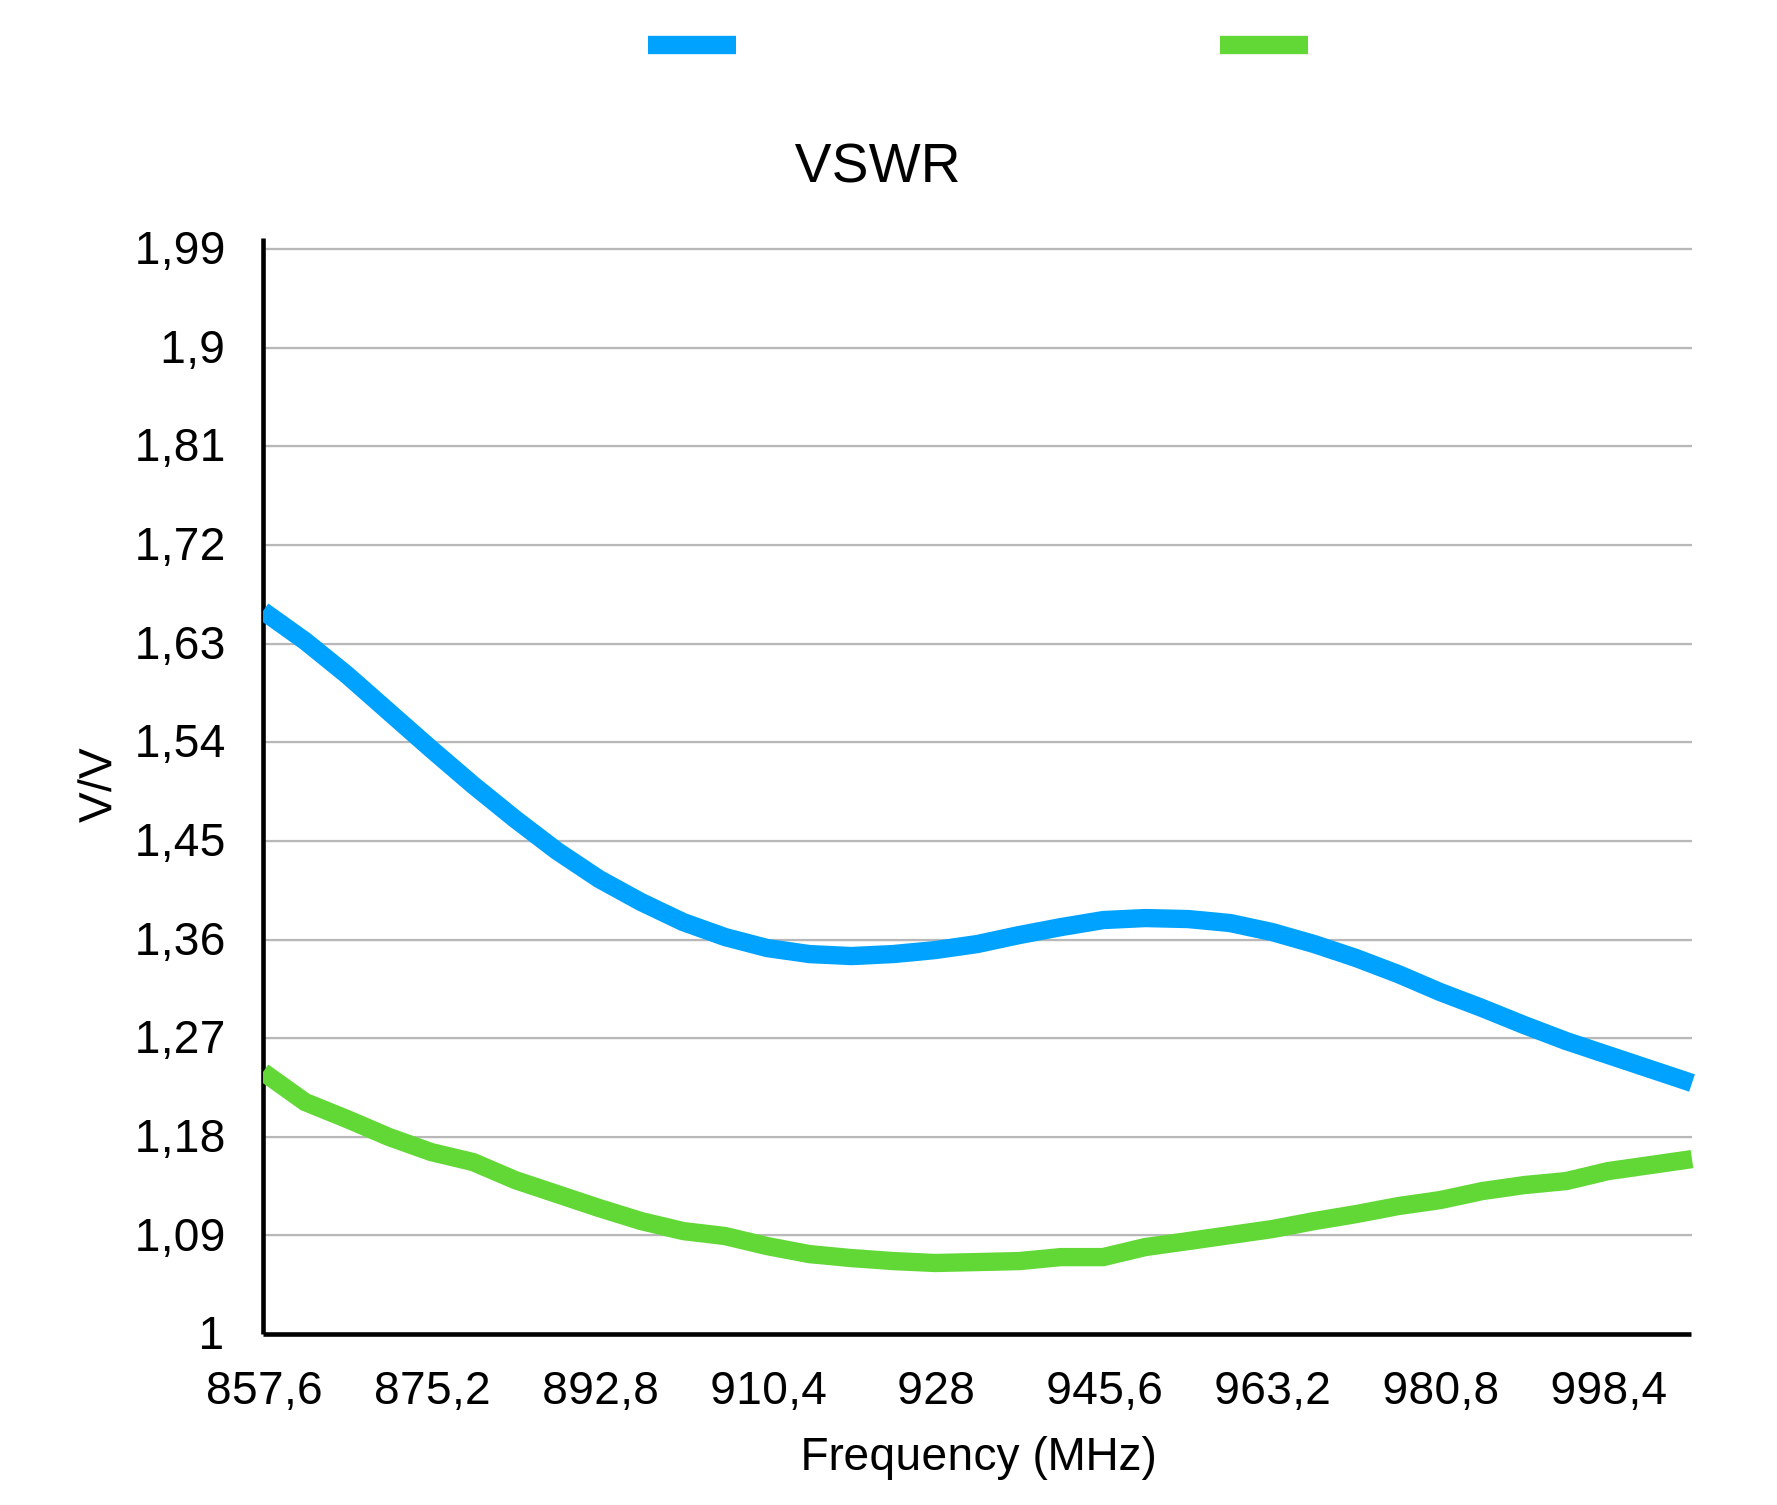
\includegraphics[width=0.9\columnwidth]{vswr-version-1}
    \caption{Comparison Test and Simulation of Antenna Version 1 VSWR}
    \label{fig9}
\end{figure}


\begin{table}[htbp]
  \begin{center}
  \caption{Antenna Version 1 RF Testing}
  \label{tab:tab8}
  \begin{tabular}{| M{0.8cm}| M{0.6cm} | M{0.6cm} |M{0.6cm} |M{0.6cm} |M{0.6cm} |M{0.6cm} |M{0.6cm} |}
      \hline
      \multirow{2}{*}{\parbox{0.8cm}{\centering $P_{out}$ Transmitter (dBm)}} & \multicolumn{7}{c|}{\centering $P_{in}$ Receiver (dBm)}\\[8pt]
      \cline{2-8}
      & 25 cm & 50 cm & 75 cm & 100 cm & 200 cm & 300 cm & 400 cm\\
      \hline
      -20 & -38.77 & -45.79 & -52.40 & -55.11 & -57.12 & -59.28 & -62.12\\
      \hline
      -10 & -29.11 & -36.13 & -43.20 & -46.90 & -49.53 & -50.89 & -58.87\\
      \hline
      0 & -19.20 & -26.48 & -34.04 & -37.37 & -41.36 & -21.01 & -50.14\\
      \hline
      10 & -8.84 & -16.38 & -24.13 & -27.55 & -31.50 & -32.71 & -45.01\\
      \hline
      20 & -2.72 & -9.22 & -15.90 & -21.41 & -23.38 & -24.33 & -39.69\\
      \hline
      30 & -2.62 & -8.88 & -16.21 & -20.60 & -25.12 & -23.57 & -35.89\\
      \hline
  \end{tabular}
  \end{center}
  \end{table}

Compared to Table~\ref{tab:tab6}, this antenna version 1 is enhanced and became a wideband antenna. It's the approach of this study to cover the changes of subtrate permittivity. Therefore, resulted a return loss of -16.664 dB, VSWR of 1.3437, and intended operating frequency, all the specifications are met but one, input impedance sheered away by 6  $\Omega$. To test it with a RF energy harvesting system, this antenna works as the receiver and the transmitter is a signal generator transmitting at different power level varied from -20 to 30 dBm. The distance between the transmitter and the receiver varied from 25 cm to 4 m. As can be seen on Table~\ref{tab:tab8}, antenna version 1 managed to receive a power of -2.62 dB at the closest distance of 25 cm with the transmitter output of 30 dBm. In the best practice, output power of 20 dBm should be enough because the higher the output power will also increase the reflected power back to the signal generator which is dangerous.


\section{Conclusion}
A wideband microstrip patch antenna has been designed and implemented. The antenna works perfectly at 915 MHz with a -16.664 dB of return loss, 1.3437 of VSWR value, and 56.3 $\Omega$ of input impedance. The techniques used are proven to be plausible to enhance the bandwidth of antenna and also the S11 parameter. However, it comes with a price where the dimension of the antenna became larger. In RF energy harvesting context, this antenna works well to cover the frequency from 756.4 MHz to 1464.8 MHz and it can forward up to -2.62 dB at the closest distance which is 25 cm with the output transmitter power of 30 dB.

% \section{Future Development}
% This antenna can be enhanced further by implementing a technique to improve the input impedance of the antenna. The closer the input impedance to 50 $\Omega$, the better the outcome is especially in harvesting the energy from the environment. Another approach that can be done is to focus on improving the gain of the antenna. However, it's going to be more complex rather than improving the S11 parameter.

\bibliographystyle{IEEEtran}
\bibliography{references}

\end{document}
